% Options for packages loaded elsewhere
\PassOptionsToPackage{unicode}{hyperref}
\PassOptionsToPackage{hyphens}{url}
\documentclass[
]{ltjsarticle}
\usepackage{xcolor}
\usepackage{amsmath,amssymb}
\setcounter{secnumdepth}{-\maxdimen} % remove section numbering
\usepackage{iftex}
\ifPDFTeX
  \usepackage[T1]{fontenc}
  \usepackage[utf8]{inputenc}
  \usepackage{textcomp} % provide euro and other symbols
\else % if luatex or xetex
  \usepackage{unicode-math} % this also loads fontspec
  \defaultfontfeatures{Scale=MatchLowercase}
  \defaultfontfeatures[\rmfamily]{Ligatures=TeX,Scale=1}
\fi
\usepackage{lmodern}
\ifPDFTeX\else
  % xetex/luatex font selection
\fi
% Use upquote if available, for straight quotes in verbatim environments
\IfFileExists{upquote.sty}{\usepackage{upquote}}{}
\IfFileExists{microtype.sty}{% use microtype if available
  \usepackage[]{microtype}
  \UseMicrotypeSet[protrusion]{basicmath} % disable protrusion for tt fonts
}{}
\makeatletter
\@ifundefined{KOMAClassName}{% if non-KOMA class
  \IfFileExists{parskip.sty}{%
    \usepackage{parskip}
  }{% else
    \setlength{\parindent}{0pt}
    \setlength{\parskip}{6pt plus 2pt minus 1pt}}
}{% if KOMA class
  \KOMAoptions{parskip=half}}
\makeatother
\usepackage{longtable,booktabs,array}
\newcounter{none} % for unnumbered tables
\usepackage{calc} % for calculating minipage widths
% Correct order of tables after \paragraph or \subparagraph
\usepackage{etoolbox}
\makeatletter
\patchcmd\longtable{\par}{\if@noskipsec\mbox{}\fi\par}{}{}
\makeatother
% Allow footnotes in longtable head/foot
\IfFileExists{footnotehyper.sty}{\usepackage{footnotehyper}}{\usepackage{footnote}}
\makesavenoteenv{longtable}
\usepackage{graphicx}
\makeatletter
\newsavebox\pandoc@box
\newcommand*\pandocbounded[1]{% scales image to fit in text height/width
  \sbox\pandoc@box{#1}%
  \Gscale@div\@tempa{\textheight}{\dimexpr\ht\pandoc@box+\dp\pandoc@box\relax}%
  \Gscale@div\@tempb{\linewidth}{\wd\pandoc@box}%
  \ifdim\@tempb\p@<\@tempa\p@\let\@tempa\@tempb\fi% select the smaller of both
  \ifdim\@tempa\p@<\p@\scalebox{\@tempa}{\usebox\pandoc@box}%
  \else\usebox{\pandoc@box}%
  \fi%
}
% Set default figure placement to htbp
\def\fps@figure{htbp}
\makeatother
\setlength{\emergencystretch}{3em} % prevent overfull lines
\providecommand{\tightlist}{%
  \setlength{\itemsep}{0pt}\setlength{\parskip}{0pt}}
\usepackage{bookmark}
\IfFileExists{xurl.sty}{\usepackage{xurl}}{} % add URL line breaks if available
\urlstyle{same}
\hypersetup{
  pdftitle={Radial Projection --- Definition and Relation to Central Projection},
  pdfauthor={Noriaki Kihara},
  hidelinks,
  pdfcreator={LaTeX via pandoc}}

\title{Radial Projection --- Definition and Relation to Central
Projection}
\usepackage{etoolbox}
\makeatletter
\providecommand{\subtitle}[1]{% add subtitle to \maketitle
  \apptocmd{\@title}{\par {\large #1 \par}}{}{}
}
\makeatother
\subtitle{A Foundational Mapping in the Central Projection Framework
(Technical Note)}
\author{Noriaki Kihara}
\date{2026-05}

\begin{document}
\maketitle

\textbf{Concept DOI (auto-redirects to the latest version)}:
\href{https://doi.org/10.5281/zenodo.20462569}{10.5281/zenodo.20462569}
\textbf{v3.3 Version DOI}:
\href{https://doi.org/10.5281/zenodo.20567347}{10.5281/zenodo.20567347}
\textbf{Zenodo page}: \url{https://zenodo.org/records/20567347}

\section{Character of This Note}\label{character-of-this-note}

\textbf{This note is a technical note that explicitly defines and
organizes the foundational mapping underlying the central projection
framework of {[}1{]}, {[}2{]}.}

The mapping treated in this note,

\[\sigma_R: \mathbb{R}^{n+1} \setminus \{0\} \to S^n(R), \quad \sigma_R(x) = \frac{R}{\|x\|} \cdot x\]

is classically known in topology as the \textbf{radial projection}, in
linear algebra and differential geometry as the \textbf{normalization
map}, and as a textbook example of a deformation retract ({[}Hatcher,
Ch. 0{]}). The note does not claim any novel geometric theorem; it only
does the following:

\begin{itemize}
\tightlist
\item
  It names this mapping \textbf{``radial projection \(\sigma_R\)''} and
  fixes the notation (§2).
\item
  It shows that the author's central projection {[}1{]} and composition
  operation {[}2{]} can be characterized as the restriction of the
  radial projection to the tangent hyperplane \(\Pi_R\) (§3).
\item
  It organizes the contrast between \(\sigma_R\) and the central
  projection \(\Phi_R\) with respect to injectivity, image, and
  differential structure (§3).
\end{itemize}

The note is not submitted to a journal; it is released as a
\textbf{Zenodo preprint that consolidates the foundations} of the
author's central projection series.

\begin{center}\rule{0.5\linewidth}{0.5pt}\end{center}

\section{§1 Introduction}\label{introduction}

\subsection{1.1 Motivation}\label{motivation}

The mapping \(x \mapsto (R/\|x\|) x\), which normalizes a vector and
sends it to the sphere of prescribed radius, is classically known in
topology as the \textbf{radial projection} (or \textbf{radial
retraction}) and in linear algebra as the \textbf{normalization map}. In
Hatcher's \emph{Algebraic Topology}, Chapter 0, for instance, it appears
as a canonical example of a deformation retract from
\(\mathbb{R}^n \setminus \{0\}\) onto \(S^{n-1}\) and is treated as one
of the most basic examples of a homotopy equivalence.

In this note we fix the symbol \(\sigma_R\) for this already-known
mapping, the symbol used within the author's central projection
framework {[}1{]}, {[}2{]}, and we collect the basic properties needed
for that framework in one place. Since many textbooks treat this mapping
only as an intermediate computation or example, an explicit note is
useful as a reference base within the series.

The purpose of this note is to name this foundational mapping ``radial
projection \(\sigma_R\)'', to fix its notation, and to make explicit its
relation to the operations appearing in the author's central projection
framework {[}1{]}, {[}2{]}.

\subsection{1.2 Relation to the Existing Central Projection
Framework}\label{relation-to-the-existing-central-projection-framework}

In the preceding paper {[}1{]} the author gave a geometric formulation
of four-dimensional spacetime via the central projection
\(\Phi_R: \Pi_R \to S^n(R)\). In {[}2{]} it was further shown that
dimension reduction operations along several axes are correctly
algebraized not as ``multiple central projections'' but as \textbf{a
single central projection together with a commuting section on the
sphere}.

This note shows that these existing central projections can be
characterized as \textbf{the restriction to the tangent hyperplane
\(\Pi_R\)} of the radial projection \(\sigma_R\), which has a larger
domain (Lemma 3.2).

A remark on orientation: the ``central projection''
\(\Phi_R: \Pi_R \to S^n(R)\) of {[}1{]} has the \textbf{opposite
orientation} to the gnomonic projection of classical cartography
(\(S^n_+ \to \Pi_R\)). In this note and in {[}1{]} we adopt the
convention that the tangent hyperplane is the source and the sphere is
the target.

\subsection{1.3 Scope of This Note}\label{scope-of-this-note}

This note treats only the following:

\begin{itemize}
\tightlist
\item
  The definition and basic properties of the radial projection
  \(\sigma_R\).
\item
  Its relation to the central projection \(\Phi_R\) (its rôle as a
  specialization).
\item
  The contrast between the image and injectivity of \(\Phi_R\) and the
  non-injectivity of \(\sigma_R\).
\end{itemize}

The following lie outside the scope of this note:

\begin{itemize}
\tightlist
\item
  Physical interpretations or applications of the radial projection
  (curvature, spacetime, quantum theory, etc.).
\item
  Concrete applications of {[}1{]}, {[}2{]} (induced metric, Einstein
  tensor, black-hole thermodynamics, etc.).
\item
  Correspondences with abstract submanifold theory such as isoparametric
  functions or polar actions.
\item
  Comparisons with other sphere-related mappings such as stereographic
  projection (which is conformal).
\end{itemize}

These will be addressed in separate notes or separate papers.

\subsection{1.4 A Note on Terminology}\label{a-note-on-terminology}

The term ``spherical projection'' is used in the literature with various
meanings (stereographic projection, various map projections, etc.). In
this note we refer to \(\sigma_R\) by the name \textbf{radial
projection}, which is the standard term in topology. To avoid confusion,
we mention this terminological choice up front.

\begin{center}\rule{0.5\linewidth}{0.5pt}\end{center}

\section{§2 Definition and Basic Properties of the Radial
Projection}\label{definition-and-basic-properties-of-the-radial-projection}

\subsection{2.1 Definition}\label{definition}

\textbf{Definition 2.1 (Radial projection).} For a positive real number
\(R > 0\), the radial projection \(\sigma_R\) is defined by

\[\sigma_R: \mathbb{R}^{n+1} \setminus \{0\} \to S^n(R), \quad \sigma_R(x) = \frac{R}{\|x\|} \cdot x \tag{2.1}\]

where \(S^n(R) = \{y \in \mathbb{R}^{n+1} \mid \|y\| = R\}\) is the
\(n\)-dimensional sphere of radius \(R\), and \(\|\cdot\|\) denotes the
standard Euclidean norm.

\textbf{Well-definedness.} Since
\(\|\sigma_R(x)\| = (R/\|x\|) \cdot \|x\| = R\), we have
\(\sigma_R(x) \in S^n(R)\).

\subsection{2.2 Basic Properties}\label{basic-properties}

\textbf{Proposition 2.1 (Basic properties).}

\begin{enumerate}
\def\labelenumi{(\roman{enumi})}
\item
  \(\sigma_R\) is of class \(C^\infty\) on the whole of
  \(\mathbb{R}^{n+1} \setminus \{0\}\) (as a smooth map into the
  submanifold \(S^n(R) \subset \mathbb{R}^{n+1}\)).
\item
  \(\sigma_R\) is a \textbf{retraction onto \(S^n(R)\)}:
  \(\sigma_R \big|_{S^n(R)} = \mathrm{id}_{S^n(R)}\). In particular, it
  is surjective.
\item
  For any \(t > 0\) and any \(x \in \mathbb{R}^{n+1} \setminus \{0\}\),
  \(\sigma_R(tx) = \sigma_R(x)\).
\end{enumerate}

\textbf{Proof.}

\begin{enumerate}
\def\labelenumi{(\roman{enumi})}
\item
  Since \(\|x\| > 0\), the map \(1/\|x\|\) is \(C^\infty\), the linear
  map \(x \mapsto x\) is \(C^\infty\), and their product is
  \(C^\infty\).
\item
  For \(y \in S^n(R)\) we have \(\|y\| = R\), hence
  \(\sigma_R(y) = (R/R) y = y\). Therefore
  \(S^n(R) \subset \mathrm{Im}(\sigma_R)\), i.e.~\(\sigma_R\) is
  surjective.
\item
  \(\sigma_R(tx) = (R/\|tx\|)(tx) = (R/(t\|x\|))(tx) = (R/\|x\|) x = \sigma_R(x)\).
  \(\square\)
\end{enumerate}

\textbf{Footnote (the case \(t < 0\)).} For \(t < 0\) one has
\(\sigma_R(tx) = -\sigma_R(x)\), so the orientation is reversed.
Property (iii) identifies only the \textbf{positive ray}
\(\{tx : t > 0\}\) emanating from the origin, not the whole line through
the origin.

\subsection{2.3 Idempotency and Retract
Structure}\label{idempotency-and-retract-structure}

\textbf{Proposition 2.2 (Idempotency).} Regarding \(\sigma_R\) as a
self-map of \(\mathbb{R}^{n+1} \setminus \{0\}\), one has
\(\sigma_R \circ \sigma_R = \sigma_R\).

\textbf{Proof.} Since \(\sigma_R(x) \in S^n(R)\), Proposition 2.1(ii)
gives \(\sigma_R(\sigma_R(x)) = \sigma_R(x)\). \(\square\)

This justifies the term ``projection'': \(\sigma_R\) is a projection
operator onto its image \(S^n(R)\).

\textbf{Deformation retract.} The homotopy
\(H(x, s) = (1-s) x + s \cdot \sigma_R(x)\) (\(s \in [0, 1]\)) realizes
a \textbf{strong deformation retract} of
\(\mathbb{R}^{n+1} \setminus \{0\}\) onto \(S^n(R)\) (classical; see
{[}Hatcher, Ch. 0{]}).

\subsection{2.4 Characterization as a Quotient
Space}\label{characterization-as-a-quotient-space}

The multiplicative group \(\mathbb{R}_{>0}\) of positive reals acts on
\(\mathbb{R}^{n+1} \setminus \{0\}\) by scalar multiplication
\(t \cdot x = tx\).

\textbf{Proposition 2.3 (Quotient space).} The quotient space

\[(\mathbb{R}^{n+1} \setminus \{0\}) / \mathbb{R}_{>0} \cong S^n(R)\]

and \(\sigma_R\) may be interpreted as the canonical section that
selects, from each positive ray (orbit), the representative point of
norm \(R\).

\textbf{Proof.} The quotient map
\(\pi: \mathbb{R}^{n+1} \setminus \{0\} \to (\mathbb{R}^{n+1} \setminus \{0\}) / \mathbb{R}_{>0}\)
and \(\sigma_R\) have the same fibers \(\{tx : t > 0\}\), so an induced
map
\(\overline{\sigma_R}: (\mathbb{R}^{n+1} \setminus \{0\}) / \mathbb{R}_{>0} \to S^n(R)\)
is well-defined and is a bijection. Continuity and smoothness are
standard. \(\square\)

This is a structural restatement of Proposition 2.1(iii); the quotient
structure makes explicit that \textbf{the radial information is
completely discarded}.

\subsection{2.5 Differential Structure}\label{differential-structure}

\textbf{Proposition 2.4 (Kernel and image of the differential).} At each
\(x \in \mathbb{R}^{n+1} \setminus \{0\}\), the differential
\(D\sigma_R|_x: \mathbb{R}^{n+1} \to T_{\sigma_R(x)} S^n(R)\) of
\(\sigma_R\) is

\[D\sigma_R|_x (v) = \frac{R}{\|x\|}\left(v - \frac{x \cdot v}{\|x\|^2} x\right) \tag{2.2}\]

and its kernel is

\[\ker D\sigma_R|_x = \mathrm{span}\{x\} \tag{2.3}\]

namely the \(x\)-direction (the radial direction). The map
\(D\sigma_R|_x\) is a submersion of rank \(n\), and its image is

\[\mathrm{Im}(D\sigma_R|_x) = x^\perp = T_{\sigma_R(x)} S^n(R) \tag{2.4}\]

(since \(\sigma_R(x)\) is a positive scalar multiple of \(x\), the
tangent space of \(S^n(R)\) at \(\sigma_R(x)\) equals the orthogonal
complement \(x^\perp\) of \(x\)).

\textbf{Proof.} Using that the directional derivative of \(\|x\|^{-1}\)
along \(v\) equals \(-\|x\|^{-3}(x \cdot v)\), differentiating
\(\sigma_R(x) = R \|x\|^{-1} x\) along \(v\) gives

\[D\sigma_R|_x(v) = R \big(-\|x\|^{-3} (x \cdot v)\big) x + R \|x\|^{-1} v = -R \|x\|^{-3} (x \cdot v) x + R \|x\|^{-1} v,\]

which rearranges to (2.2). For the kernel, setting
\(D\sigma_R|_x(v) = 0\) yields

\[v - \frac{x \cdot v}{\|x\|^2} x = 0,\]

hence

\[v = \frac{x \cdot v}{\|x\|^2} x,\]

so \(v\) is a scalar multiple of \(x\). Conversely, if
\(v = \lambda x\), then

\[v - \frac{x \cdot v}{\|x\|^2} x = \lambda x - \frac{\lambda \|x\|^2}{\|x\|^2} x = 0,\]

so \(D\sigma_R|_x(v) = 0\). Therefore
\(\ker D\sigma_R|_x = \mathrm{span}\{x\}\).

For the image, for any \(v\) we have
\(x \cdot D\sigma_R|_x(v) = \frac{R}{\|x\|}\left(x \cdot v - \frac{x \cdot v}{\|x\|^2}\|x\|^2\right) = 0\),
so \(\mathrm{Im}(D\sigma_R|_x) \subseteq x^\perp\). By the rank--nullity
theorem,
\(\dim \mathrm{Im}(D\sigma_R|_x) = (n+1) - \dim \ker D\sigma_R|_x = n = \dim x^\perp\),
hence \(\mathrm{Im}(D\sigma_R|_x) = x^\perp = T_{\sigma_R(x)} S^n(R)\).
\(\square\)

This clarifies the differential-geometric structure of the radial
projection: \textbf{the radial direction corresponds exactly to the
kernel of the differential, and only the tangential directions are
mapped onto the sphere}.

\subsection{2.6 Preservation of Angles Between
Vectors}\label{preservation-of-angles-between-vectors}

\textbf{Proposition 2.5 (Preservation of angles).} For any
\(x, y \in \mathbb{R}^{n+1} \setminus \{0\}\),

\[\angle(\sigma_R(x), \sigma_R(y)) = \angle(x, y) \tag{2.5}\]

where \(\angle(\cdot, \cdot)\) denotes the unoriented angle between
vectors.

\textbf{Proof.}

\[\frac{\sigma_R(x) \cdot \sigma_R(y)}{\|\sigma_R(x)\| \cdot \|\sigma_R(y)\|} = \frac{(R/\|x\|)(R/\|y\|)(x \cdot y)}{R \cdot R} = \frac{x \cdot y}{\|x\| \cdot \|y\|},\]

so the cosines agree and the angles are equal. \(\square\)

\textbf{Remark (terminology).} This is the preservation of the angle
between two vectors and is a different notion from conformality
(preservation of angles between curves). Since \(\sigma_R\) drops
dimension, preservation of angles between curves is not even meaningful
for it.

\subsection{2.7 Scale Invariance}\label{scale-invariance}

\textbf{Proposition 2.6 (Invariance of direction under radius
rescaling).} For any \(R_1, R_2 > 0\) and any
\(x \in \mathbb{R}^{n+1} \setminus \{0\}\), the points
\(\sigma_{R_1}(x)\) and \(\sigma_{R_2}(x)\) lie on the same positive ray
from the origin \(O\) through \(x\).

\textbf{Proof.} Both \(\sigma_{R_1}(x) = (R_1/\|x\|) x\) and
\(\sigma_{R_2}(x) = (R_2/\|x\|) x\) are positive scalar multiples of
\(x\). \(\square\)

That is, in the radial projection \textbf{the directional component is
invariant under rescaling of the radius \(R\)}.

\begin{figure}
\centering
\pandocbounded{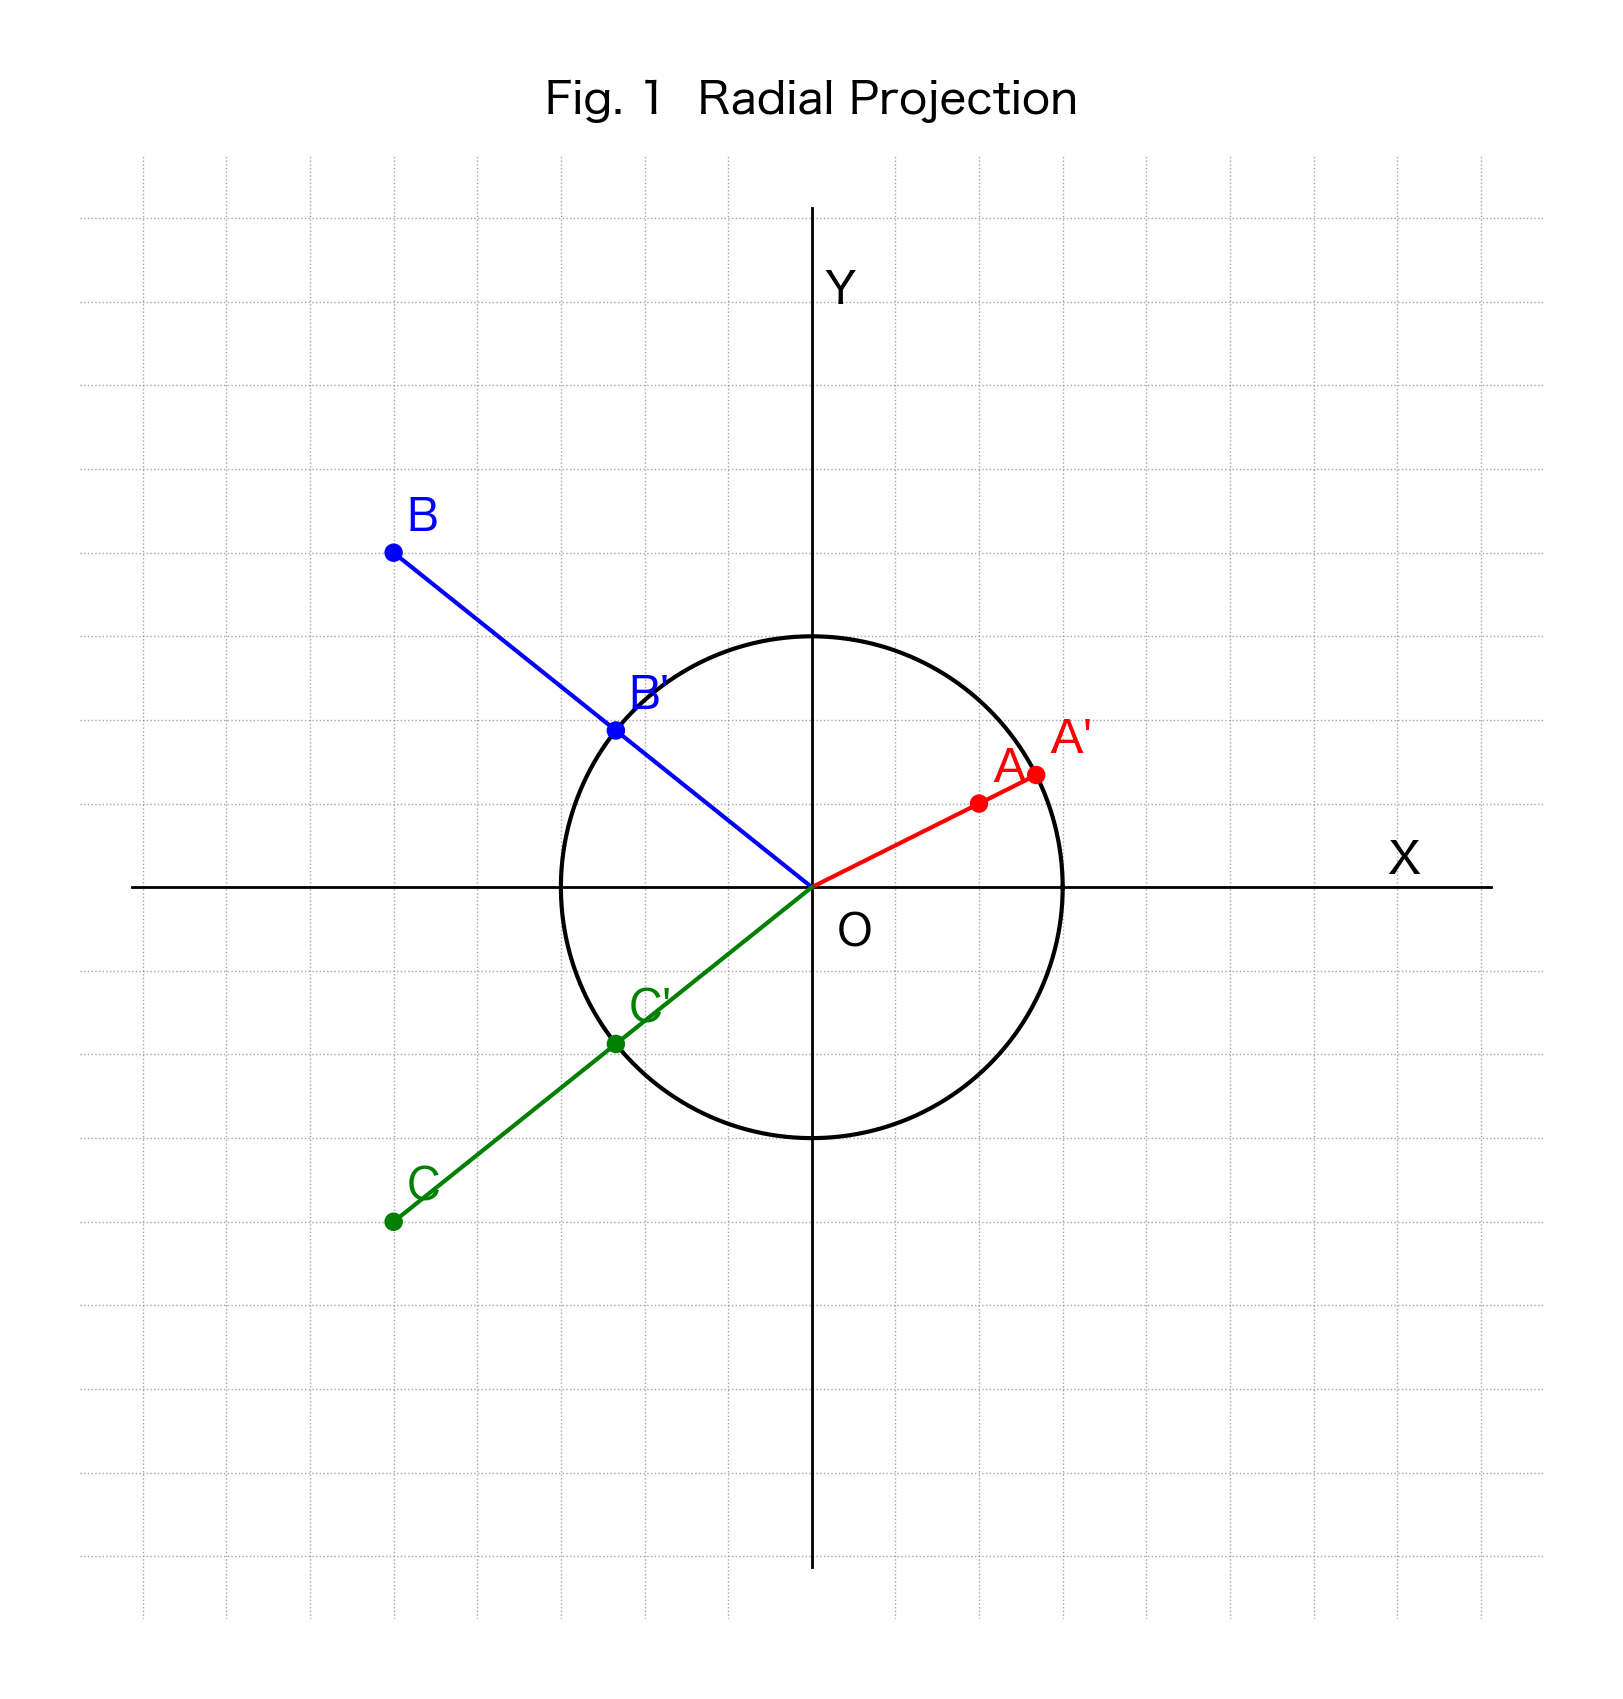
\includegraphics[keepaspectratio,alt={Fig. 1 Radial Projection}]{fig1_radial_projection.png}}
\caption{Fig. 1 Radial Projection}
\end{figure}

\textbf{Fig. 1}: Illustration of the radial projection \(\sigma_R\)
(\(n=1\), \(R=3\)). With the origin \(O\) as the viewpoint, the points
\(A\) (inside the circle) and \(B, C\) (outside the circle, in different
quadrants) on radial rays are sent to the points \(A', B', C'\) on the
circle.

\begin{figure}
\centering
\pandocbounded{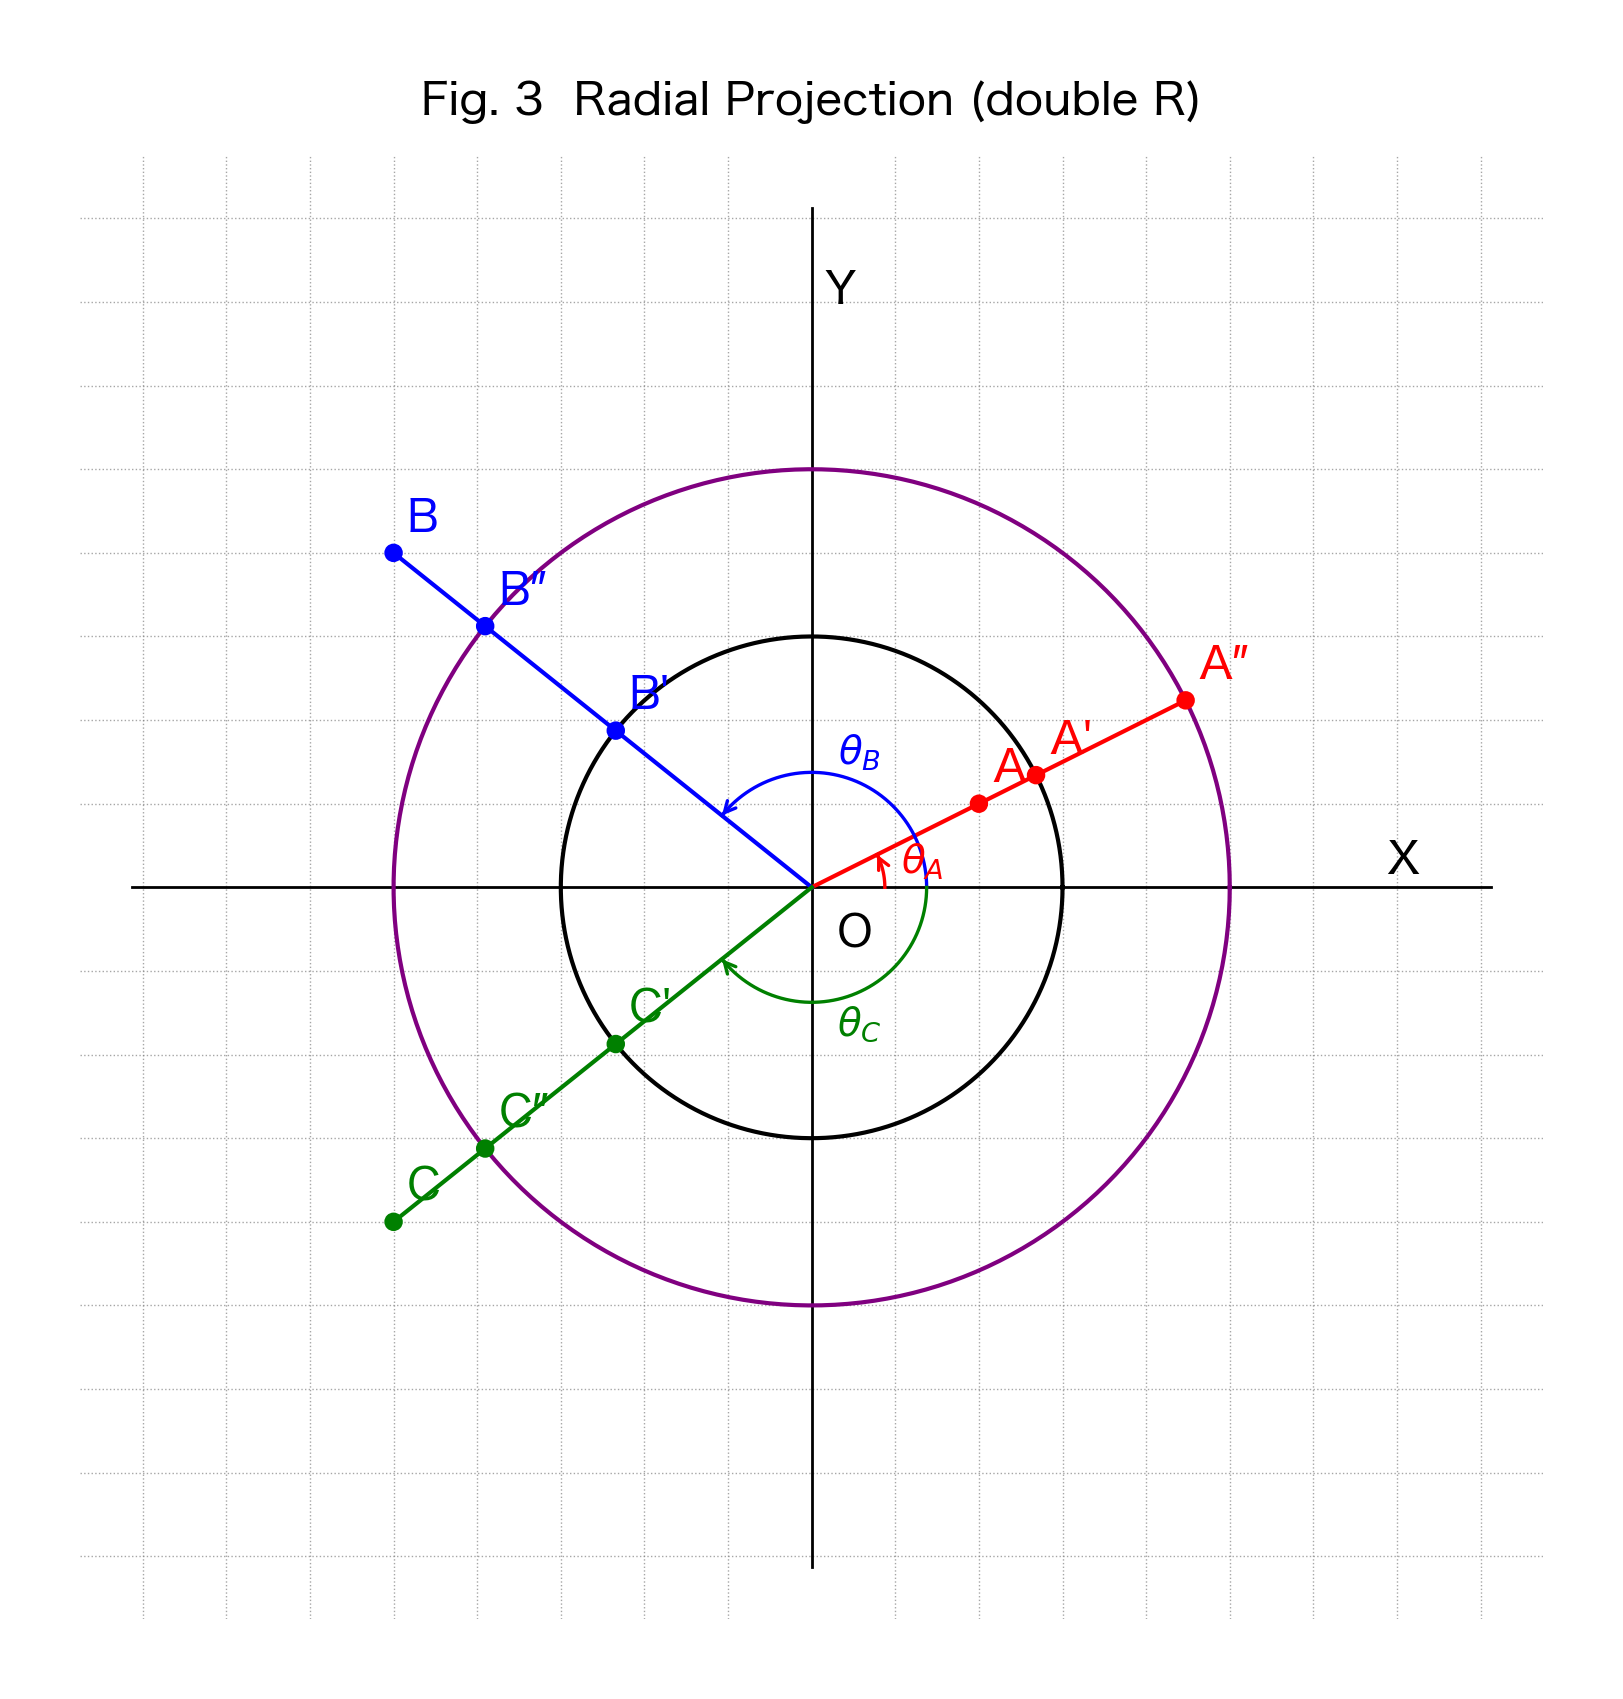
\includegraphics[keepaspectratio,alt={Fig. 3 Radial Projection (double R)}]{fig3_radial_projection_double_R.png}}
\caption{Fig. 3 Radial Projection (double R)}
\end{figure}

\textbf{Fig. 3}: Invariance of direction under radius rescaling in the
radial projection (Proposition 2.6). For both radii \(R=3\) (black
circle) and \(R=5\) (purple circle), the images of \(A, B, C\) lie on
the same radial rays. Consequently the angles
\(\theta_A, \theta_B, \theta_C\) that each point makes with the positive
\(x\)-axis are preserved independently of \(R\).

\subsection{2.8 A Distortion Invisible for a Single Point, Manifest for
Several
Points}\label{a-distortion-invisible-for-a-single-point-manifest-for-several-points}

Propositions 2.5 (angle preservation) and 2.6 (invariance of direction
under radius rescaling) state that \(\sigma_R\) preserves the direction
of each point, while Propositions 2.3 and 2.4 state that the radial
information is completely discarded. Combining these, we obtain the
following elementary observation about the character of the distortion
induced by \(\sigma_R\).

\textbf{Observation 2.7 (Relational nature of the distortion).} Focusing
on a single point \(x\) alone, \(\sigma_R(x) = (R/\|x\|)\,x\) merely
normalizes \(x\) to radius \(R\) along the same positive ray
(Proposition 2.6), and its action is indistinguishable from a scale
transformation. That \(\sigma_R\) does \textbf{not} preserve distances
(spacings) \textbf{cannot be observed from the image of a single point}.

By contrast, focusing on several distinct points \(x_1, \ldots, x_m\),
each point is normalized by a \textbf{different factor \(R/\|x_i\|\)}
according to its own norm, so the spacings (arc length or chord length)
between the images \(\sigma_R(x_i)\) on the sphere do not, in general,
agree with the Euclidean spacings between the original points. In
particular, a sequence of points \textbf{equally spaced} on the tangent
hyperplane \(\Pi_R\) is mapped by \(\sigma_R\) (\(= \Phi_R\), Lemma 3.2)
to a \textbf{non-equally-spaced} sequence on the sphere (Fig. 4). That
is, the distortion of \(\sigma_R\) is not an attribute of a single
point; \textbf{it becomes manifest only as a relation (relative
configuration, spacing) between points.}

This is an elementary, visualizable manifestation of the fact that
\(\sigma_R\) preserves angles (Proposition 2.5) and directions
(Proposition 2.6) while failing to preserve distances. The aspect of
formulating this spacing distortion as an induced metric or curvature
lies outside the scope of this note (§1.3, §4.3) and is treated in the
separate papers {[}1{]}, {[}2{]}.

\begin{figure}
\centering
\pandocbounded{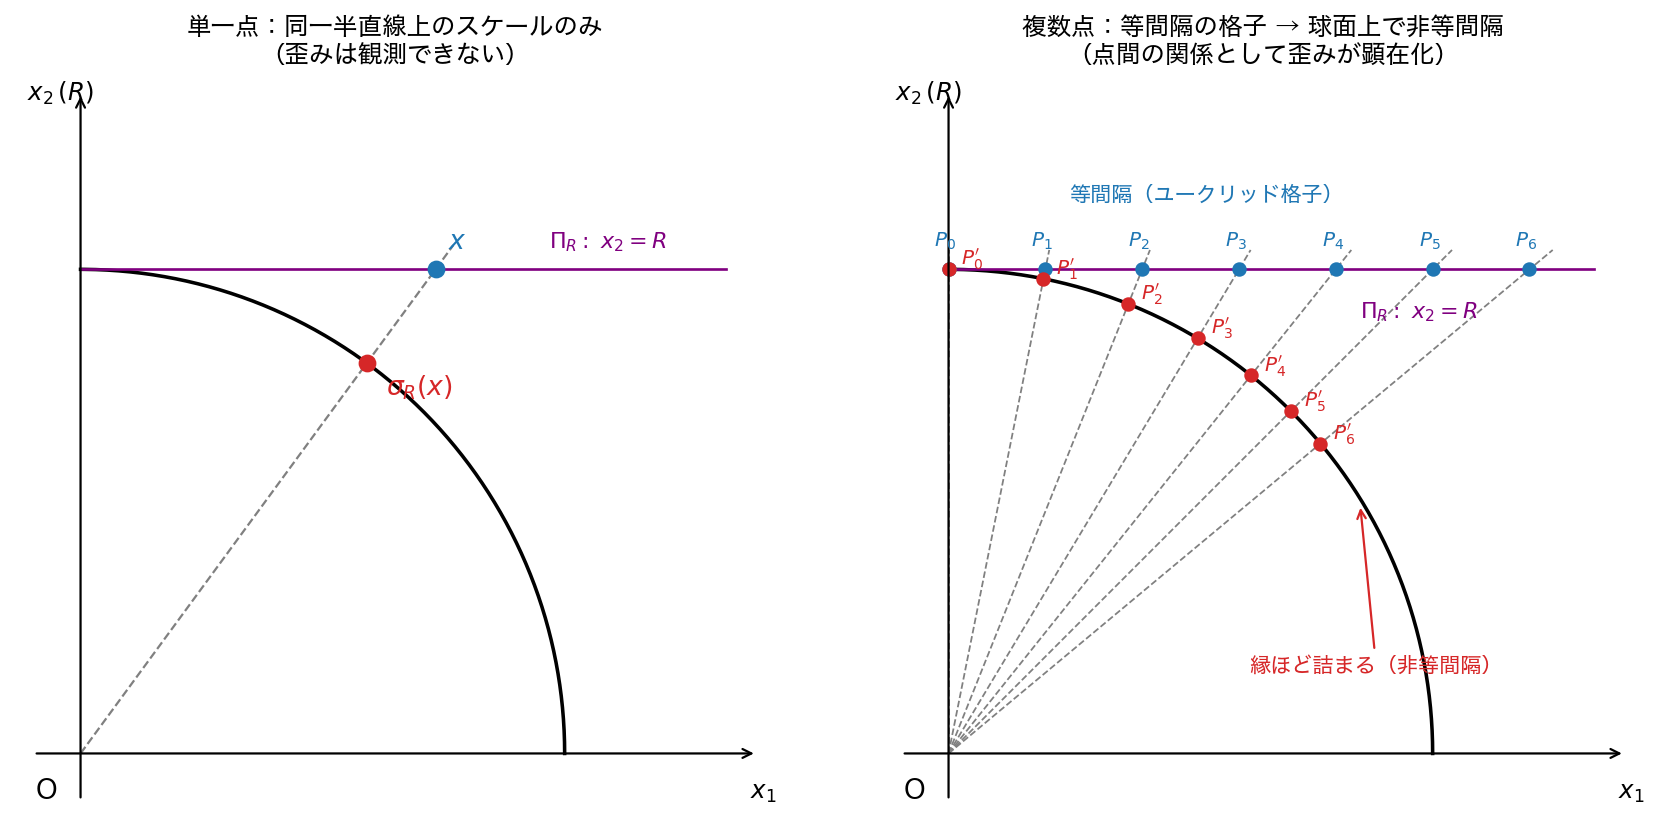
\includegraphics[keepaspectratio,alt={Fig. 4 Radial Projection (spacing distortion)}]{fig4_radial_projection_spacing.png}}
\caption{Fig. 4 Radial Projection (spacing distortion)}
\end{figure}

\textbf{Fig. 4}: Relational nature of the distortion in the radial
projection (\(n=1\), \(R=3\)). (Left) A single point \(x\): its image
\(\sigma_R(x)\) lies on the same radial ray, and the action is
indistinguishable from a scale transformation. (Right) A sequence of
points \(P_0, \ldots, P_6\) equally spaced on the tangent hyperplane
\(\Pi_R\) is mapped to a non-equally-spaced sequence
\(P_0', \ldots, P_6'\) on the sphere (the larger the angle---toward the
edge---the more they crowd together). The distortion becomes manifest
only as the spacing between points.

\begin{center}\rule{0.5\linewidth}{0.5pt}\end{center}

\section{§3 Relation to the Central
Projection}\label{relation-to-the-central-projection}

\subsection{3.1 Definition of the Central
Projection}\label{definition-of-the-central-projection}

\textbf{Definition 3.1 (Central projection).} Let the tangent hyperplane
at the north pole \(N = (0, \ldots, 0, R)\) of the sphere \(S^n(R)\) be

\[\Pi_R = \{x \in \mathbb{R}^{n+1} \mid x_{n+1} = R\}. \tag{3.1}\]

We have \(\Pi_R \cong \mathbb{R}^n\). The central projection \(\Phi_R\)
is defined by

\[\Phi_R: \Pi_R \to S^n_+(R), \quad \Phi_R(x) = \frac{R}{\|x\|} \cdot x \tag{3.2}\]

where \(S^n_+(R) = \{y \in S^n(R) \mid y_{n+1} > 0\}\) is the
\textbf{open upper hemisphere}. That this is the image of \(\Phi_R\) is
shown in Proposition 3.1 below.

This agrees with the central projection defined in §2 of {[}1{]} (for
the positivity of the final coordinate, see Remark 3.1 of {[}1{]}).

\textbf{Remark (on orientation).} The present \(\Phi_R\) has the
orientation \textbf{tangent hyperplane (source) \(\to\) sphere
(target)}. The gnomonic projection of classical cartography is often
defined in the opposite direction (sphere \(\to\) tangent plane), so the
terminological mismatch should be kept in mind.

\subsection{3.2 Image and Injectivity of the Central
Projection}\label{image-and-injectivity-of-the-central-projection}

\textbf{Proposition 3.1 (Image and injectivity of \(\Phi_R\)).}

\begin{enumerate}
\def\labelenumi{(\roman{enumi})}
\item
  The image of \(\Phi_R\) is the open upper hemisphere
  \(S^n_+(R) = \{y \in S^n(R) \mid y_{n+1} > 0\}\).
\item
  \(\Phi_R: \Pi_R \to S^n_+(R)\) is a \textbf{diffeomorphism} (in
  particular, injective).
\end{enumerate}

\textbf{Proof.}

\begin{enumerate}
\def\labelenumi{(\roman{enumi})}
\item
  For \(x \in \Pi_R\) we have \(x_{n+1} = R\), so the last coordinate of
  \(\Phi_R(x)\) is \((R/\|x\|) \cdot R = R^2/\|x\| > 0\). Hence
  \(\Phi_R(\Pi_R) \subset S^n_+(R)\). Conversely, given any
  \(y \in S^n_+(R)\) with \(y_{n+1} > 0\), set \(x := (R/y_{n+1}) y\);
  then \(x_{n+1} = R\), so \(x \in \Pi_R\),
  \(\|x\| = R\|y\|/y_{n+1} = R^2/y_{n+1}\), and
  \(\Phi_R(x) = (R/\|x\|) x = (y_{n+1}/R) \cdot (R/y_{n+1}) y = y\).
  Hence \(\Phi_R\) is surjective onto \(S^n_+(R)\).
\item
  The construction in (i) furnishes the inverse
  \(\Phi_R^{-1}(y) = (R/y_{n+1}) y\), which is \(C^\infty\) in both
  directions. \(\square\)
\end{enumerate}

\subsection{3.3 Relation Between the Radial Projection and the Central
Projection}\label{relation-between-the-radial-projection-and-the-central-projection}

\textbf{Lemma 3.2 (The central projection is a restriction of the radial
projection).} The central projection \(\Phi_R\) coincides with the
radial projection \(\sigma_R\) when the domain is restricted to
\(\Pi_R\) and the codomain is restricted to \(S^n_+(R)\):

\[\Phi_R = \sigma_R \big|_{\Pi_R}: \Pi_R \to S^n_+(R). \tag{3.3}\]

\textbf{Proof.} The defining formulas \(\sigma_R(x) = (R/\|x\|) x\)
(Definition 2.1) and \(\Phi_R(x) = (R/\|x\|) x\) (Definition 3.1) are
identical. Moreover \(\Pi_R \subset \mathbb{R}^{n+1} \setminus \{0\}\)
(since on \(\Pi_R\) we have \(x_{n+1} = R > 0\), so no point of
\(\Pi_R\) is the origin), and restricting the domain of \(\sigma_R\) to
\(\Pi_R\) gives \(\Phi_R\). That the image lies in \(S^n_+(R)\) follows
from Proposition 3.1(i). \(\square\)

\subsection{\texorpdfstring{3.4 Contrast Between \(\sigma_R\) and
\(\Phi_R\)}{3.4 Contrast Between \textbackslash sigma\_R and \textbackslash Phi\_R}}\label{contrast-between-sigma_r-and-phi_r}

{\def\LTcaptype{none} % do not increment counter
\begin{longtable}[]{@{}
  >{\raggedright\arraybackslash}p{(\linewidth - 4\tabcolsep) * \real{0.3333}}
  >{\raggedright\arraybackslash}p{(\linewidth - 4\tabcolsep) * \real{0.3333}}
  >{\raggedright\arraybackslash}p{(\linewidth - 4\tabcolsep) * \real{0.3333}}@{}}
\toprule\noalign{}
\begin{minipage}[b]{\linewidth}\raggedright
Property
\end{minipage} & \begin{minipage}[b]{\linewidth}\raggedright
\(\sigma_R\)
\end{minipage} & \begin{minipage}[b]{\linewidth}\raggedright
\(\Phi_R\)
\end{minipage} \\
\midrule\noalign{}
\endhead
\bottomrule\noalign{}
\endlastfoot
Domain & \(\mathbb{R}^{n+1} \setminus \{0\}\) & \(\Pi_R\) (tangent
hyperplane, isomorphic to \(\mathbb{R}^n\)) \\
Image & \(S^n(R)\) (whole sphere) & \(S^n_+(R)\) (\textbf{open upper
hemisphere only}) \\
Injectivity & \textbf{Non-injective} (each ray collapses to a point) &
\textbf{Injective} (diffeomorphism) \\
Radial direction & Contained in the kernel (Proposition 2.4) & The
kernel direction is not contained in the domain's tangent space
(transversal) \\
\end{longtable}
}

This contrast is the \textbf{core} of the present note. The radial
projection extends the domain to all of
\(\mathbb{R}^{n+1} \setminus \{0\}\) at the cost of losing injectivity.
The central projection, on the other hand, retains injectivity and the
rich geometric structure (induced metric, curvature, etc.) but its
domain is restricted to \(\Pi_R\) and its image to \(S^n_+(R)\).

\begin{figure}
\centering
\pandocbounded{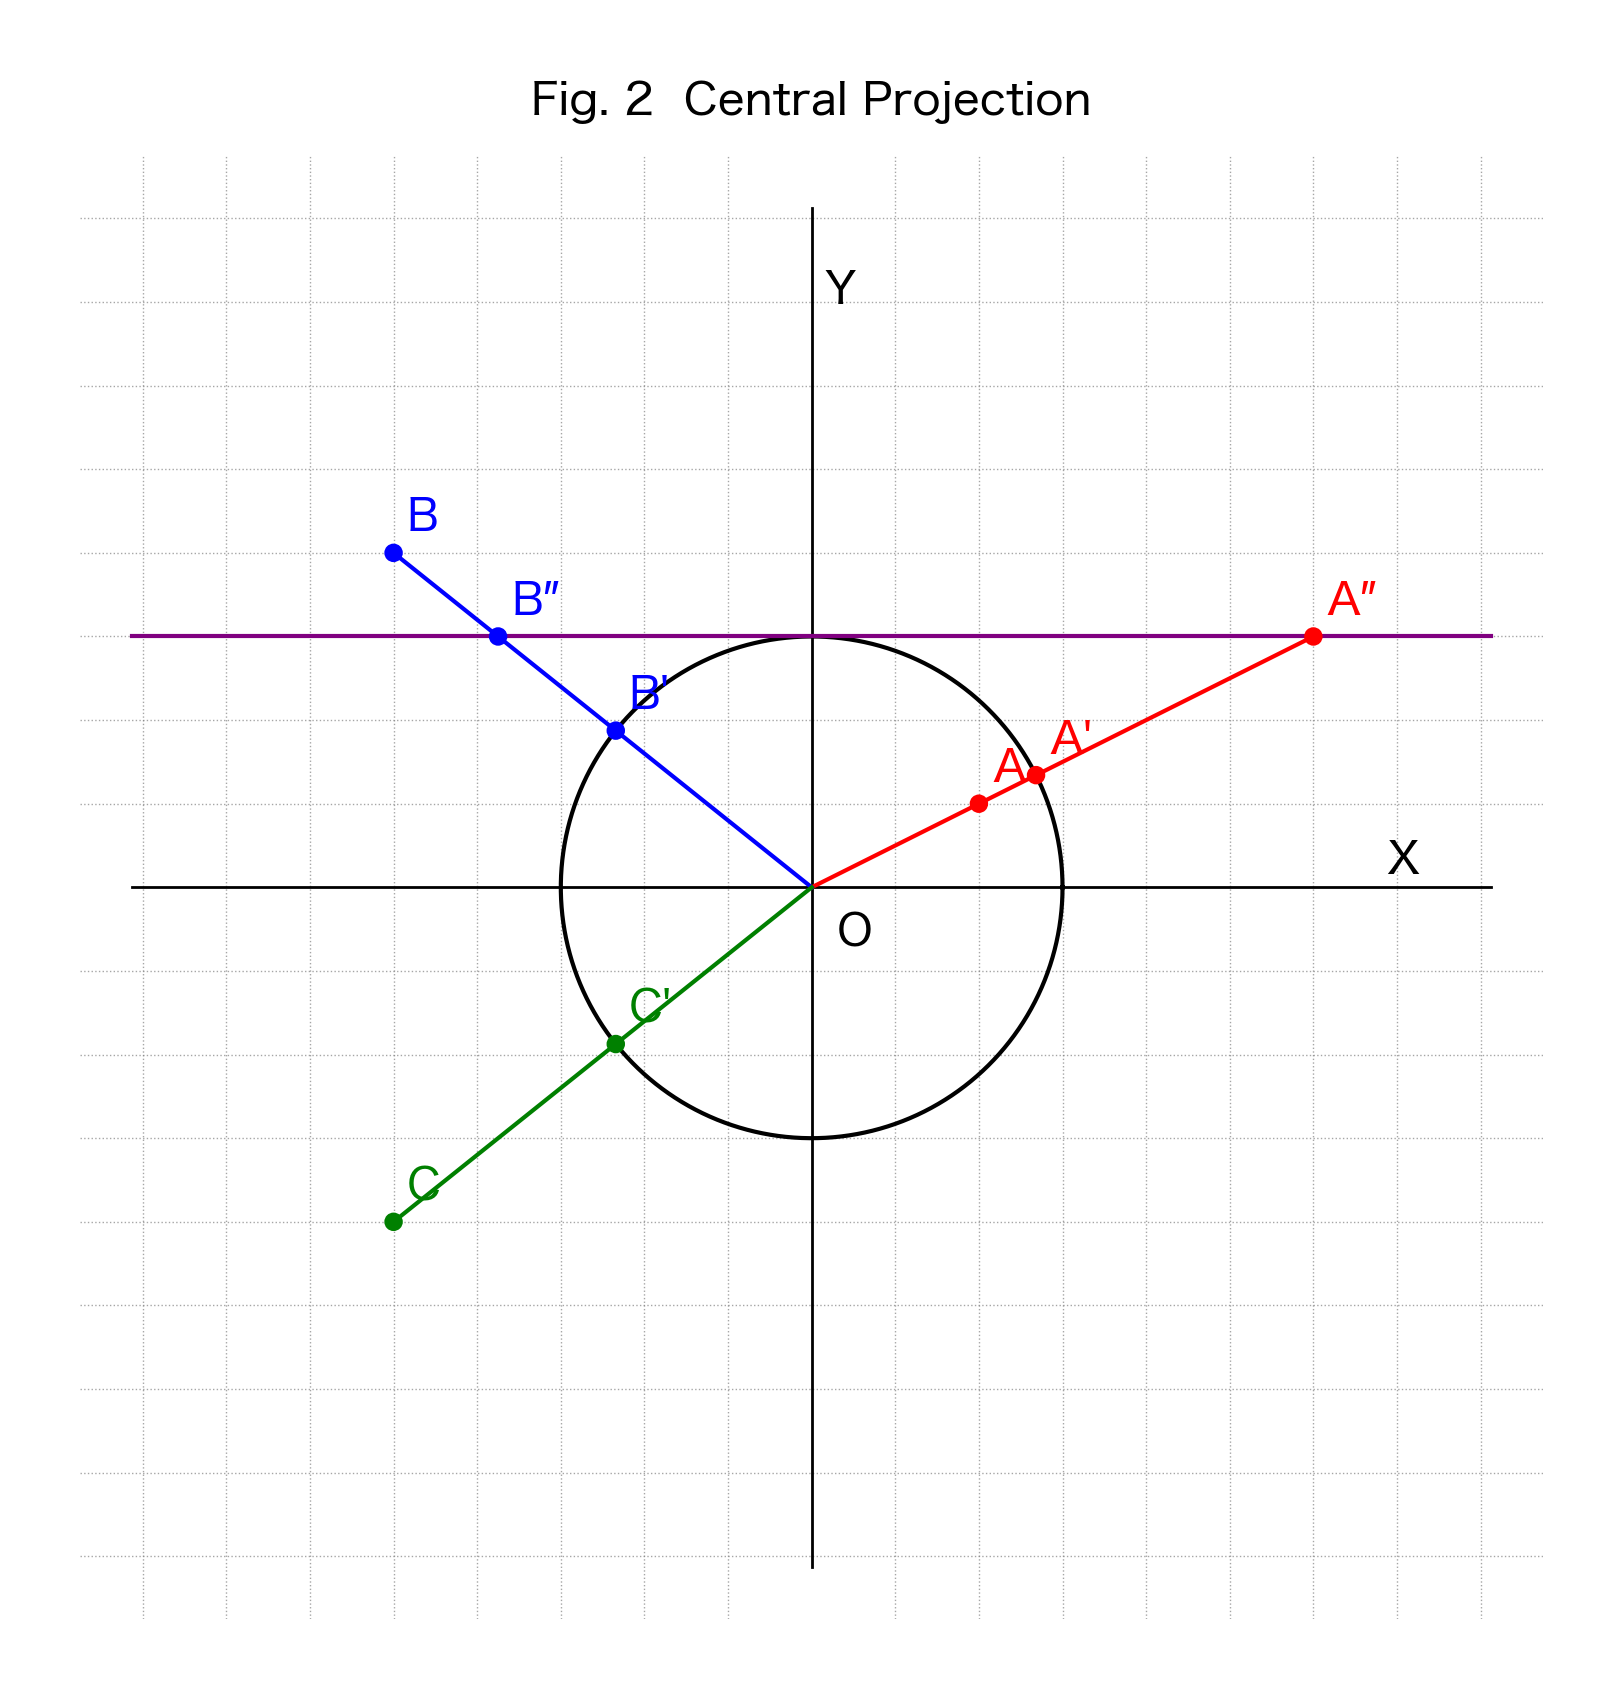
\includegraphics[keepaspectratio,alt={Fig. 2 Central Projection}]{fig2_central_projection.png}}
\caption{Fig. 2 Central Projection}
\end{figure}

\textbf{Fig. 2}: Illustration of the central projection \(\Phi_R\)
(\(n=1\), \(R=3\)). The points \(A'', B''\) on the tangent hyperplane
(purple line; for \(n=1\) this is the line \(y = R\), and in general it
is \(x_{n+1} = R\) as in (3.1)) tangent to the sphere at the north pole
are projected onto \(A', B'\) on the sphere along radial rays from the
origin \(O\). The radial projection \(\sigma_R\) is defined along the
very same rays, and the sole difference between the two is their domain.
The image of \(\Phi_R\) is the open upper hemisphere (it does not reach
the lower hemisphere, nor does it reach the equator from any finite
point). The green pair \(C, C'\) is an example of the radial projection
\(\sigma_R\) and is not contained in the image of the central projection
\(\Phi_R\) (the open upper hemisphere).

\subsection{3.5 Relation to Existing
Results}\label{relation-to-existing-results}

\textbf{Remark 3.1 (Rewriting of existing results).} The geometric
quantities defined via \(\Phi_R\) in {[}1{]} and {[}2{]} (the induced
metric \(g_{\mu\nu} = \Phi_R^* g_{S^n(R)}\), the Einstein tensor, the
composite curvature radius
\(r_{\text{final}}^2 = r_1^2 - \sum_{j \in S}(x_{i_j}^*)^2\), and so on)
can be rewritten in the notation of this note as pullbacks under
\(\sigma_R \big|_{\Pi_R}\).

However, these geometric quantities are intrinsically structures on
\(\Pi_R\) (mapping into the upper hemisphere) and do not extend
automatically to the extended domain of the radial projection
\(\sigma_R\). For a general smooth map \(f: M \to N\), the pullback
\(f^* T\) is well-defined regardless of injectivity; in particular
\(\sigma_R^* g_{S^n(R)}\) is a well-defined symmetric 2-tensor on
\(\mathbb{R}^{n+1} \setminus \{0\}\). But, by Proposition 2.4, the
radial direction \(\mathrm{span}\{x\}\) lies in the kernel of the
differential, so this pullback tensor is degenerate and is not a
Riemannian metric. Hence it cannot be identified with the non-degenerate
induced metric that \(\Phi_R^* g_{S^n(R)}\) gives on \(\Pi_R\).

The semigroup structure, commutativity, and closed form of the composite
curvature radius for the section operation of {[}2{]} (which, to avoid
notational collision in this note, we denote \(\kappa_S\)) are
positioned as operations on the image space \(S^n(R)\) of \(\sigma_R\).

\begin{center}\rule{0.5\linewidth}{0.5pt}\end{center}

\section{§4 Conclusion}\label{conclusion}

\subsection{4.1 Main Results of This
Note}\label{main-results-of-this-note}

\begin{enumerate}
\def\labelenumi{\arabic{enumi}.}
\tightlist
\item
  We have explicitly defined the radial projection
  \(\sigma_R(x) = (R/\|x\|) x\) as a \(C^\infty\) retraction from
  \(\mathbb{R}^{n+1} \setminus \{0\}\) onto \(S^n(R)\) (Definition 2.1,
  Proposition 2.1).
\item
  We have organized at an elementary level its idempotency, deformation
  retract structure, quotient-space description, kernel and image of the
  differential, angle preservation, and scale invariance (Propositions
  2.2--2.6). Furthermore, we made explicit, as an observation, the
  relational property that the distortion of \(\sigma_R\) does not
  appear for a single point but becomes manifest only as the spacing
  between several points (Observation 2.7, Fig. 4).
\item
  The central projection \(\Phi_R\) is equal to the restriction of the
  radial projection \(\sigma_R\) to the tangent hyperplane \(\Pi_R\),
  its image is the \textbf{open upper hemisphere \(S^n_+(R)\)}, and
  \(\Phi_R\) is a diffeomorphism (Definition 3.1, Proposition 3.1, Lemma
  3.2).
\item
  The contrast between the non-injectivity of \(\sigma_R\) and the
  injectivity of \(\Phi_R\) has been collected in §3.4.
\end{enumerate}

\subsection{4.2 Position}\label{position}

The radial projection \(\sigma_R\) defined in this note is identical to
the mapping classically known in topology as the \textbf{radial
projection} (see e.g.~{[}Hatcher, Ch. 0{]}). The contribution of this
note is not the discovery of a new geometric theorem; it is limited to

\begin{itemize}
\tightlist
\item
  explicitly naming and fixing the notation for this foundational
  mapping as the ``radial projection \(\sigma_R\)'', and
\item
  making explicit its relation to the operations appearing in the
  author's central projection framework {[}1{]}, {[}2{]}.
\end{itemize}

This note is released as a \textbf{Zenodo preprint / technical note} to
consolidate the foundations of the central projection series; submission
to a pure-mathematics journal is not intended.

\subsection{4.3 What This Note Does Not
Claim}\label{what-this-note-does-not-claim}

\begin{itemize}
\tightlist
\item
  That the radial projection \(\sigma_R\) was ``undiscovered in prior
  work'' (it is classically known as the radial projection).
\item
  Any deep mathematical result about \(\sigma_R\) (general
  correspondences with submanifold theory, polar actions, isoparametric
  functions, conformality, and so on).
\item
  That the rich geometric structure of the central projection \(\Phi_R\)
  (induced metric, curvature tensors, etc.) is automatically inherited
  by \(\sigma_R\) via the mere domain extension (in fact, since
  injectivity is lost, the pullback is well-defined only when restricted
  to \(\Pi_R\) in the relevant non-degenerate sense).
\item
  Any physical application, cosmological interpretation, or
  quantum-theoretic implication.
\end{itemize}

These are addressed in separate notes or separate papers.

\begin{center}\rule{0.5\linewidth}{0.5pt}\end{center}

\section{References}\label{references}

{[}1{]} Kihara, N. (2026). \emph{Geometric Formulation of
Four-Dimensional Space via Central Projection}. Zenodo. Concept DOI:
\href{https://doi.org/10.5281/zenodo.19427780}{10.5281/zenodo.19427780}.

{[}2{]} Kihara, N. (2026). \emph{Composition of Central Projections and
a Closed Form for the Composite Curvature Radius: An Algebraic
Formulation of Higher-Dimensional Reduction via One Central Projection
and Commuting Sections on the Sphere}. Zenodo. Concept DOI:
\href{https://doi.org/10.5281/zenodo.20060728}{10.5281/zenodo.20060728}.

{[}3{]} A. Hatcher (2002). \emph{Algebraic Topology}. Cambridge
University Press. (Chapter 0: the deformation retract
\(r(x) = x/\|x\|\).)

\begin{center}\rule{0.5\linewidth}{0.5pt}\end{center}

Author: Noriaki Kihara Affiliation: WF System Co., Ltd. ORCID:
\href{https://orcid.org/0009-0004-6753-4020}{0009-0004-6753-4020}
License: CC BY 4.0

\begin{center}\rule{0.5\linewidth}{0.5pt}\end{center}

\subsection{Revision History}\label{revision-history}

\begin{itemize}
\tightlist
\item
  \textbf{v1 (2026-05-30, first draft)}: initial version.
\item
  \textbf{v2 (2026-05-30, revision)}: integrated the comments from a
  4-AI peer review (Claude.ai, ChatGPT, Gemini, Grok):

  \begin{itemize}
  \tightlist
  \item
    Naming: keep ``radial projection \(\sigma_R\)'' while stating in §1
    that this is ``the same as the topological radial projection''.
  \item
    Position: explicitly framed as a technical note / Zenodo preprint.
  \item
    Image of the central projection explicitly identified as the open
    upper hemisphere \(S^n_+(R)\) (Proposition 3.1).
  \item
    ``Angle preservation'' was tightened to genuine preservation of
    angles between vectors (Proposition 2.5, inner-product formula) and
    the scale-invariance statement was separated out (Proposition 2.6).
  \item
    New propositions added: idempotency (Proposition 2.2), quotient
    space (Proposition 2.3), kernel of the differential (Proposition
    2.4).
  \item
    Claims about being a ``higher-level concept'' or about ``the absence
    of a standard text'' were weakened.
  \item
    The previous Corollary 3.1(ii) was downgraded to Remark 3.1 and made
    self-contained.
  \item
    Added the external reference Hatcher (reference {[}3{]}).
  \item
    The symbol \(\sigma_S\) was renamed \(\kappa_S\) for the section
    operation of {[}2{]}.
  \item
    ``Phase'' replaced by ``directional component'' throughout.
  \item
    The case \(t < 0\) is now treated in a footnote.
  \item
    The orientation mismatch between the central projection \(\Phi_R\)
    and the classical gnomonic projection is now explicitly noted in
    §1.2 and §3.1.
  \item
    Well-definedness is now stated immediately after the definition.
  \end{itemize}
\item
  \textbf{v3 (2026-05-30, minor revision)}: reflected the second-round
  comments from ChatGPT on v2:

  \begin{itemize}
  \tightlist
  \item
    The proof of the kernel in Proposition 2.4 was rewritten correctly
    (now in the ``equivalence between \(D\sigma_R|_x(v)=0\) and
    \(v=\lambda x\)'' form).
  \item
    In Remark 3.1 (§3.5), ``the pullback is not well-defined'' was
    corrected to ``the pullback is well-defined but degenerate'' (the
    pullback of a tensor is always well-defined, independently of
    injectivity; the issue is degeneracy).
  \item
    The caption of Fig. 3 was corrected so that it refers only to
    Proposition 2.6 (Proposition 2.5 removed).
  \item
    The caption of Fig. 2 was supplemented to note that the green pair
    \(C, C'\) is not in the image of the central projection.
  \item
    In §1.1, the phrasing ``no standalone document exists for it as a
    primary named operation'' was weakened to ``useful as a reference
    base within the series''.
  \item
    The caption of Fig. 2 was supplemented with ``for \(n=1\) this is
    \(y = R\), and in general it is \(x_{n+1} = R\) as in (3.1)'' (per
    Gemini's second-round comment).
  \end{itemize}
\item
  \textbf{v3.1 (2026-05-30, minor revision)}: reflected the minor
  comments from Claude.ai's second-round review of v2:

  \begin{itemize}
  \tightlist
  \item
    Added to Proposition 2.4 the image of the differential
    \(\mathrm{Im}(D\sigma_R|_x) = x^\perp = T_{\sigma_R(x)} S^n(R)\)
    (equation (2.4)). This makes the submersion structure more explicit
    and records that the tangent space of the sphere at \(\sigma_R(x)\)
    equals the orthogonal complement of the radial direction.
  \end{itemize}
\item
  \textbf{v3.3 (2026-06-06, content addition; English draft)}: added a
  new §2.8 ``A Distortion Invisible for a Single Point, Manifest for
  Several Points'' (Observation 2.7, Fig. 4). In a purely geometric
  register, it makes explicit that \(\sigma_R\) preserves angles
  (Proposition 2.5) and directions (Proposition 2.6) while failing to
  preserve distances (spacings): for a single point the action is
  indistinguishable from a scale transformation and the distortion
  cannot be observed, whereas an equally-spaced sequence on the tangent
  hyperplane \(\Pi_R\) maps to a non-equally-spaced sequence on the
  sphere (crowding toward the edge), so the distortion becomes manifest
  only as a relation between points. Added Fig. 4 (a two-panel
  single-point vs.~several-points comparison). Physical interpretation
  (curvature, spacetime, motion) remains outside the scope (§1.3, §4.3)
  and is deferred to {[}1{]}, {[}2{]}. §4.1 main results updated to
  include Observation 2.7. \textbf{Japanese/English md, tex, and pdf
  were regenerated, and the note was published as a new Zenodo version
  preserving the Concept DOI (10.5281/zenodo.20462569); Version DOI:
  10.5281/zenodo.20567347.}
\item
  \textbf{v3.2 (2026-06-02, copy-editing)}: reflected copy-editing and
  polishing comments from peer review:

  \begin{itemize}
  \tightlist
  \item
    Resolved a duplicate equation number: the angle-preservation
    identity in Proposition 2.5 was renumbered from (2.4) to
    \textbf{(2.5)} (it had collided with the image equation (2.4) of
    Proposition 2.4).
  \item
    The cross-reference in §1.2 was already correct (``Lemma 3.2'');
    verified consistent with §3.3 and §4.1.
  \item
    Added to the proof of Proposition 2.4 the \textbf{argument for the
    image \(\mathrm{Im} = x^\perp\)} (via
    \(x \cdot D\sigma_R|_x(v) = 0\) and the rank--nullity theorem);
    previously only the kernel was justified.
  \item
    Renamed the heading of Proposition 2.4 from ``Kernel of the
    differential'' to ``\textbf{Kernel and image of the differential}''
    (consistent with its content); §4.1 item 2 updated likewise.
  \item
    Tightened the \(\Phi_R\) ``radial direction'' cell of the §3.4 table
    from ``no radial direction in the domain'' to ``\textbf{the kernel
    direction is not contained in the domain's tangent space
    (transversal)}''.
  \item
    Clarified the opening of the Proposition 2.4 proof: replaced the
    ambiguous \(\frac{d}{dx}\) notation with a \textbf{directional
    derivative along \(v\)}.
  \end{itemize}
\end{itemize}

\end{document}
